\documentclass[a4paper,12pt,twocolumn]{article}

\usepackage[landscape,top=1cm,bottom=1.4cm,left=1cm,right=1cm,columnsep=1cm]{geometry}
\usepackage[fleqn]{amsmath}
\usepackage{amssymb}
\setlength{\mathindent}{1.5em}
\usepackage{fontspec}
\usepackage{enumitem}
\usepackage{framed}
\usepackage{xeCJK}
\usepackage{needspace}
\usepackage[hidelinks]{hyperref}
\usepackage{tikz}

\setmainfont{Times New Roman}
\setsansfont{Arial}
\setmonofont{JetBrains Mono}

% Chinese font support
\setCJKmainfont{Iansui}[
  BoldFont=Iansui,
  AutoFakeBold=3.17
]

\pagestyle{plain}
\setlength{\columnseprule}{0.2pt}
\newcommand{\examdate}{2026/04/17}
\newlength{\problemnumberwidth}
\settowidth{\problemnumberwidth}{\textbf{69.}\ }
\newenvironment{solutionbox}{\begin{framed}}{\end{framed}}

\newcommand{\sectiontitle}[2]{%
  \hypertarget{#1}{}%
  \par\vspace{0.8em}%
  \noindent{\Large\bfseries #2}\par
  \vspace{0.3em}%
  \hrule
  \vspace{0.8em}%
}

\newcommand{\tocproblem}[2]{%
  \hyperref[#1]{#2} & \hyperref[#1]{\pageref*{#1}} \\
}

\newcommand{\worksheettoc}{%
  \noindent{\Large\bfseries Contents}\par
  \vspace{0.3em}%
  \hrule
  \vspace{0.9em}%
  \begin{tabular}{@{}p{0.72\columnwidth}r@{}}
    \textbf{Problem} & \textbf{Page} \\
    \tocproblem{prob:13-1-41}{13-1 \quad 41}
    \tocproblem{prob:13-1-42}{13-1 \quad 42}
    \tocproblem{prob:13-1-43}{13-1 \quad 43}
    \tocproblem{prob:13-1-44}{13-1 \quad 44}
    \tocproblem{prob:13-1-45}{13-1 \quad 45}
    \tocproblem{prob:13-1-46}{13-1 \quad 46}
    \tocproblem{prob:13-1-57}{13-1 \quad 57}
    \tocproblem{prob:13-1-59}{13-1 \quad 59}
    \tocproblem{prob:13-1-60}{13-1 \quad 60}
    \tocproblem{prob:13-2-24}{13-2 \quad 24}
    \tocproblem{prob:13-2-28}{13-2 \quad 28}
    \tocproblem{prob:13-2-29}{13-2 \quad 29}
    \tocproblem{prob:13-2-35}{13-2 \quad 35}
    \tocproblem{prob:13-2-52}{13-2 \quad 52}
  \end{tabular}\par
}

\newcommand{\problem}[3]{%
  \Needspace{10\baselineskip}%
  \phantomsection\label{#1}%
  \par\vspace{0.8em}%
  \noindent
  \hangindent=\problemnumberwidth
  \hangafter=1
  \makebox[\problemnumberwidth][l]{\textbf{#2.}}#3\par
}

\newlist{subparts}{enumerate}{1}
\setlist[subparts]{%
  label = (\alph*),
  labelindent=\problemnumberwidth,
  leftmargin=*,
  labelsep=0.5em,
  align=left,
  itemsep=0.2em,
  topsep=0.3em,
  parsep=0pt,
  partopsep=0pt
}

\newlist{steps}{enumerate}{1}
\setlist[steps]{%
  label=\textbf{Step \arabic*.},
  leftmargin=*,
  itemsep=0.35em,
  topsep=0.35em,
  align=left
}

\begin{document}

\twocolumn[
{\centering
\Large\bfseries Calculus Problems Solutions\par
\vspace{0.5em}
\noindent\hfill\normalsize\normalfont \examdate\par
\vspace{0.8em}
}
]

\worksheettoc
\vfill\null
\newpage

\sectiontitle{sec:13-1}{13-1}

\problem{prob:13-1-41}{41}{Graph the curve with the given vector equation.
\[
r(t)=\langle \cos t\sin 2t,\ \sin t\sin 2t,\ \cos 2t\rangle
\]}

\begin{solutionbox}
\textbf{Method 1: Identify the surface first, then read the projection}

\begin{steps}
\item Rewrite the coordinates as
\[
x=\sin 2t\cos t,\qquad y=\sin 2t\sin t,\qquad z=\cos 2t.
\]
This is the right first step because the factors \(\sin 2t\) and \(\cos 2t\) suggest a hidden trigonometric identity.

\item Compute
\[
x^2+y^2+z^2
=\sin^2 2t(\cos^2 t+\sin^2 t)+\cos^2 2t
=1.
\]
So the curve lies on the unit sphere. That immediately tells us the graph is not an arbitrary space curve: it is constrained to the sphere.

\item Next look at the projection onto the \(xy\)-plane. Written in signed polar form,
\[
r=\sin 2t,\qquad \theta=t.
\]
Thus the \(xy\)-projection is the rose
\[
r=\sin 2\theta,
\]
which has four petals. If one insists on the standard nonnegative polar radius, then
\[
\rho=\sqrt{x^2+y^2}=|\sin 2t|,
\]
and whenever \(\sin 2t<0\), the same point is represented by replacing the angle \(t\) with \(t+\pi\). This is appropriate because the top view usually reveals how the curve winds around the \(z\)-axis.

\item Now combine the two facts. The curve stays on the sphere while its top view traces a four-petaled rose. Also
\[
z=\cos 2t,
\]
so the point starts at the north pole when \(t=0\), reaches the south pole when \(t=\pi/2\), returns to the north pole when \(t=\pi\), and repeats this behavior once more before \(t=2\pi\).

\item Therefore a good domain is \(0\le t\le 2\pi\). Over this interval the curve is a closed spherical rose: it runs on the sphere and meets the poles at
\[
t=0,\ \frac{\pi}{2},\ \pi,\ \frac{3\pi}{2},\ 2\pi.
\]
\end{steps}
\end{solutionbox}

\begin{solutionbox}
\textbf{Method 2: Recognize it as a spherical-coordinate parametrization}

\begin{steps}
\item Compare the curve with the standard spherical-coordinate form
\[
x=\sin\phi\cos\theta,\qquad y=\sin\phi\sin\theta,\qquad z=\cos\phi.
\]
Matching terms gives
\[
\phi=2t,\qquad \theta=t.
\]
This method is appropriate because the given formula already looks exactly like the spherical-coordinate template.

\item The equation \(\phi=2t\) means the polar angle changes twice as fast as the azimuth angle. So while the point turns once around the \(z\)-axis, it moves from pole to pole and back.

\item Some key positions confirm the shape:
\[
t=0 \Rightarrow (0,0,1),\qquad
t=\frac{\pi}{4}\Rightarrow \left(\frac{\sqrt2}{2},\frac{\sqrt2}{2},0\right),
\]
\[
t=\frac{\pi}{2}\Rightarrow (0,0,-1),\qquad
t=\frac{3\pi}{4}\Rightarrow \left(\frac{\sqrt2}{2},-\frac{\sqrt2}{2},0\right),
\]
\[
t=\pi \Rightarrow (0,0,1).
\]
These checkpoints show the curve alternates between equatorial petals and the poles.

\item Since both \(\sin 2t\) and \(\cos 2t\) have period \(2\pi\) in the full vector expression, the curve closes over \(0\le t\le 2\pi\).
\end{steps}
\end{solutionbox}

\begin{solutionbox}
\textbf{Hand-in Version}

The curve can be written as
\[
x=\sin 2t\cos t,\qquad y=\sin 2t\sin t,\qquad z=\cos 2t.
\]
Hence
\[
x^2+y^2+z^2=\sin^2 2t+\cos^2 2t=1,
\]
so it lies on the unit sphere.

Its projection onto the \(xy\)-plane can be written in signed polar form as
\[
r=\sin 2t,\qquad \theta=t,
\]
so the top view is the four-petaled rose \(r=\sin 2\theta\). Equivalently, with the standard nonnegative radius,
\[
\rho=|\sin 2t|,
\]
and the angle is shifted by \(\pi\) whenever \(\sin 2t<0\). Also \(z=\cos 2t\), so the curve moves from the north pole to the south pole and back twice while the azimuth angle turns once around the sphere.

Therefore, for \(0\le t\le 2\pi\), the graph is a closed spherical rose on the unit sphere.

\begin{center}
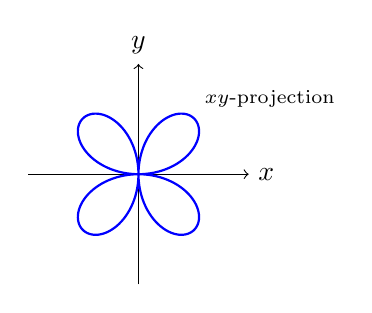
\begin{tikzpicture}[scale=1.0]
\draw[->] (-1.4,0) -- (1.4,0) node[right] {\(x\)};
\draw[->] (0,-1.4) -- (0,1.4) node[above] {\(y\)};
\draw[thick,blue,domain=0:360,samples=240,smooth,variable=\t]
  plot ({sin(2*\t)*cos(\t)},{sin(2*\t)*sin(\t)});
\node[above right] at (0.72,0.72) {\scriptsize \(xy\)-projection};
\end{tikzpicture}
\end{center}
\end{solutionbox}

\problem{prob:13-1-42}{42}{Graph the curve with the given vector equation.
\[
r(t)=\langle te^t,\ e^{-t},\ t\rangle
\]}

\begin{solutionbox}
\textbf{Method 1: Eliminate the parameter and view the curve as an intersection}

\begin{steps}
\item Because the third coordinate is \(z=t\), the easiest elimination starts with
\[
t=z.
\]
Then
\[
y=e^{-t}=e^{-z},
\qquad
x=te^t=ze^z.
\]
This is appropriate because \(z=t\) gives an immediate substitution.

\item A second useful relation comes from multiplying the first two coordinates:
\[
xy=(te^t)(e^{-t})=t=z.
\]
So the curve lies on the saddle surface
\[
z=xy
\]
and also on the exponential cylinder
\[
y=e^{-z}.
\]
The graph is therefore the intersection of two simpler surfaces.

\item Now describe the motion. Since \(z=t\), the curve rises steadily as \(t\) increases. Also
\[
y=e^{-t}>0
\]
for every \(t\), so the entire curve stays in the half-space \(y>0\).

\item The endpoints at infinity are also clear:
\[
t\to-\infty \Rightarrow (x,y,z)\to(0^{-},\infty,-\infty),
\]
\[
t\to\infty \Rightarrow (x,y,z)\to(\infty,0^{+},\infty).
\]
So the curve is open, not closed, and it runs from far up in the positive \(y\)-direction down toward the plane \(y=0\) while rising in \(z\).
\end{steps}
\end{solutionbox}

\begin{solutionbox}
\textbf{Method 2: Read the shape from the three coordinate projections}

\begin{steps}
\item In the \(yz\)-plane, eliminate \(t\) using \(z=t\):
\[
y=e^{-z}.
\]
This is a decreasing exponential. It tells us immediately that the curve always moves toward smaller \(y\) as \(z\) increases.

\item In the \(xz\)-plane,
\[
x=ze^z.
\]
Differentiating gives
\[
\frac{dx}{dz}=e^z(z+1),
\]
so \(x\) has its unique minimum at \(z=-1\), where
\[
x=-\frac1e.
\]
This explains why the curve first bends slightly into negative \(x\) and then turns strongly toward positive \(x\).

\item In the \(xy\)-plane, use \(y=e^{-t}\), so \(t=-\ln y\). Then
\[
x=te^t=\frac{t}{y}=-\frac{\ln y}{y},\qquad y>0.
\]
This shows the top view is also open and remains entirely above the \(x\)-axis in the \(xy\)-plane.

\item The curve passes through
\[
t=0 \Rightarrow (0,1,0),
\]
which is the most natural checkpoint for sketching. A practical plotting window such as \(-2\le t\le 2\) shows the essential bend, but the true domain is all real \(t\).
\end{steps}
\end{solutionbox}

\begin{solutionbox}
\textbf{Hand-in Version}

Since \(z=t\), we have
\[
y=e^{-z},\qquad x=ze^z.
\]
Also
\[
xy=(te^t)(e^{-t})=t=z.
\]
So the curve is the intersection of
\[
\boxed{z=xy}
\qquad\text{and}\qquad
\boxed{y=e^{-z}.}
\]

It is an open space curve with \(y>0\) for all \(t\), passing through \((0,1,0)\). As \(t\to-\infty\), the curve approaches \((0^{-},\infty,-\infty)\); as \(t\to\infty\), it approaches \((\infty,0^{+},\infty)\). The \(yz\)-projection is the exponential \(y=e^{-z}\), and the \(xz\)-projection is \(x=ze^z\) with minimum \(x=-1/e\) at \(z=-1\).
\end{solutionbox}

\problem{prob:13-1-43}{43}{Graph the curve with the given vector equation.
\[
r(t)=\left\langle \sin 3t\cos t,\ \frac{t}{4},\ \sin 3t\sin t\right\rangle
\]}

\begin{solutionbox}
\textbf{Method 1: Use the projection onto the \(xz\)-plane}

\begin{steps}
\item The \(x\)- and \(z\)-coordinates are
\[
x=\sin 3t\cos t,\qquad z=\sin 3t\sin t.
\]
So in signed polar form in the \(xz\)-plane,
\[
r=\sin 3t,\qquad \theta=t.
\]
That means the \(xz\)-projection is the three-petaled rose
\[
r=\sin 3\theta.
\]
If one wants the standard nonnegative radius, then
\[
\rho=\sqrt{x^2+z^2}=|\sin 3t|,
\]
and when \(\sin 3t<0\), the same projected point is obtained by increasing the angle by \(\pi\). This is the right place to start because the entire oscillation of the curve is carried by the \(x\)- and \(z\)-coordinates.

\item The remaining coordinate is
\[
y=\frac{t}{4},
\]
which increases linearly with \(t\). So the rose-shaped projection is not repeated in a single plane: it is lifted upward at constant speed as \(t\) increases.

\item Therefore the curve is an open ``rose helix'' about the \(y\)-axis. Every time the \(xz\)-projection draws one full three-petaled rose, the curve rises by
\[
\Delta y=\frac{2\pi}{4}=\frac{\pi}{2}.
\]
This gives the correct large-scale shape.

\item The curve passes through the \(y\)-axis whenever \(\sin 3t=0\), that is,
\[
t=\frac{n\pi}{3}
\quad\Longrightarrow\quad
(x,z)=(0,0),\qquad y=\frac{n\pi}{12}.
\]
So the curve repeatedly threads through the \(y\)-axis as it climbs.
\end{steps}
\end{solutionbox}

\begin{solutionbox}
\textbf{Method 2: Package the horizontal motion in a complex number}

\begin{steps}
\item Write
\[
x+iz=\sin 3t(\cos t+i\sin t)=\sin 3t\,e^{it}.
\]
This form is useful because it separates the horizontal radius \(\sin 3t\) from the turning angle \(t\).

\item The factor \(e^{it}\) means the point rotates around the \(y\)-axis with angular speed \(1\), while \(\sin 3t\) makes the distance from the \(y\)-axis expand and collapse three times as fast.

\item Since \(y=t/4\), the curve never closes in space. A good representative domain is \(0\le t\le 2\pi\): over that interval the \(xz\)-projection completes one full three-petal rose while \(y\) rises from \(0\) to \(\pi/2\).

\item Key points help anchor the sketch:
\[
t=0\Rightarrow (0,0,0),\qquad
t=\frac{\pi}{6}\Rightarrow \left(\frac{\sqrt3}{2},\frac{\pi}{24},\frac12\right),
\]
\[
t=\frac{\pi}{2}\Rightarrow \left(0,\frac{\pi}{8},-1\right),\qquad
t=\pi\Rightarrow \left(0,\frac{\pi}{4},0\right).
\]
These show how the petals occur at increasing heights.
\end{steps}
\end{solutionbox}

\begin{solutionbox}
\textbf{Hand-in Version}

The \(xz\)-projection is
\[
x=\sin 3t\cos t,\qquad z=\sin 3t\sin t,
\]
so in signed polar coordinates it is
\[
\boxed{r=\sin 3\theta.}
\]
Equivalently, with standard nonnegative radius,
\[
\rho=|\sin 3t|,
\]
and the angle must be shifted by \(\pi\) whenever \(\sin 3t<0\). Thus the top view relative to the \(y\)-axis is a three-petaled rose.

Since
\[
y=\frac{t}{4},
\]
the curve rises linearly while the \(xz\)-projection repeats the rose pattern. Therefore the graph is an open rose-shaped helix about the \(y\)-axis, crossing the \(y\)-axis whenever \(t=n\pi/3\).

A representative viewing window is \(0\le t\le 2\pi\), which shows one full rose while \(y\) increases by \(\pi/2\).

\begin{center}
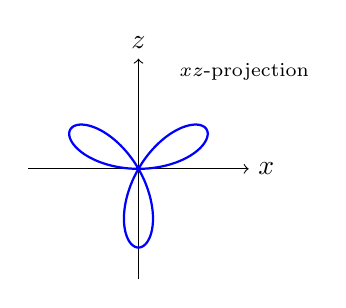
\begin{tikzpicture}[scale=1.0]
\draw[->] (-1.4,0) -- (1.4,0) node[right] {\(x\)};
\draw[->] (0,-1.4) -- (0,1.4) node[above] {\(z\)};
\draw[thick,blue,domain=0:360,samples=240,smooth,variable=\t]
  plot ({sin(3*\t)*cos(\t)},{sin(3*\t)*sin(\t)});
\node[above right] at (0.4,1.0) {\scriptsize \(xz\)-projection};
\end{tikzpicture}
\end{center}
\end{solutionbox}

\problem{prob:13-1-44}{44}{Graph the curve with the given vector equation.
\[
r(t)=\langle \cos(8\cos t)\sin t,\ \sin(8\cos t)\sin t,\ \cos t\rangle
\]}

\begin{solutionbox}
\textbf{Method 1: Find the supporting surface and the longitude rule}

\begin{steps}
\item Let
\[
x=\cos(8\cos t)\sin t,\qquad
y=\sin(8\cos t)\sin t,\qquad
z=\cos t.
\]
Then
\[
x^2+y^2=\sin^2 t.
\]
Therefore
\[
x^2+y^2+z^2=\sin^2 t+\cos^2 t=1.
\]
So the curve lies on the unit sphere.

\item On \(0\le t\le \pi\), we have \(\sin t\ge 0\), so ordinary cylindrical coordinates apply:
\[
\rho=\sin t=\sqrt{1-z^2},
\qquad
\theta=8\cos t=8z.
\]
This shows that as the point moves down the sphere, its longitude changes according to \(\theta=8z\). That is exactly the description of a spherical spiral.

\item When \(t=0\), the point is \((0,0,1)\), the north pole. When \(t=\pi\), the point is \((0,0,-1)\), the south pole. Between them, the longitude changes from \(8\) to \(-8\), so the point winds around the sphere about
\[
\frac{16}{2\pi}\approx 2.55
\]
times before reaching the south pole.

\item Over \(\pi\le t\le 2\pi\), the factor \(\sin t\) changes sign. In standard cylindrical coordinates the radius must remain nonnegative, so we rewrite this part as
\[
\rho=|\sin t|,\qquad \theta=8\cos t+\pi.
\]
That is, the negative sign in \(\sin t\) is absorbed by a \(\pi\)-shift in the azimuth angle. Geometrically, this means the curve returns to the north pole along the opposite side of the sphere. Thus \(0\le t\le 2\pi\) gives the full closed curve.
\end{steps}
\end{solutionbox}

\begin{solutionbox}
\textbf{Method 2: Trace key checkpoints and use symmetry}

\begin{steps}
\item Important points are
\[
t=0\Rightarrow (0,0,1),\qquad
t=\frac{\pi}{2}\Rightarrow (1,0,0),\qquad
t=\pi\Rightarrow (0,0,-1),
\]
\[
t=\frac{3\pi}{2}\Rightarrow (-1,0,0),\qquad
t=2\pi\Rightarrow (0,0,1).
\]
These anchor the curve at the poles and at two opposite equatorial points.

\item The factor \(\cos(8\cos t)\) and \(\sin(8\cos t)\) means the azimuth depends on \(\cos t=z\), not directly on \(t\). So the direction around the \(z\)-axis is controlled by height. This is why the curve wraps around the sphere instead of behaving like an ordinary latitude or longitude circle.

\item Since the curve starts at the north pole, spirals down to the south pole, then returns to the north pole, the true shape is a closed spherical spiral with two pole-to-pole branches.
\end{steps}
\end{solutionbox}

\begin{solutionbox}
\textbf{Hand-in Version}

Because
\[
x^2+y^2=\sin^2 t,\qquad z=\cos t,
\]
we have
\[
x^2+y^2+z^2=1,
\]
so the curve lies on the unit sphere.

For \(0\le t\le \pi\),
\[
\rho=\sin t=\sqrt{1-z^2},
\qquad
\theta=8\cos t=8z,
\]
so the point spirals from the north pole to the south pole while its longitude changes according to \(\theta=8z\). For \(\pi\le t\le 2\pi\), the standard cylindrical description is
\[
\rho=|\sin t|,\qquad \theta=8\cos t+\pi,
\]
so the negative sign is absorbed into the angle and the curve returns along the opposite side before closing up.

Hence, on \(0\le t\le 2\pi\), the graph is a closed spherical spiral on the unit sphere.
\end{solutionbox}

\problem{prob:13-1-45}{45}{Graph the curve with the given vector equation.
\[
r(t)=\langle \cos 2t,\ \cos 3t,\ \cos 4t\rangle
\]}

\begin{solutionbox}
\textbf{Method 1: Eliminate the parameter as far as possible}

\begin{steps}
\item Let \(u=\cos t\). Then
\[
x=\cos 2t=2u^2-1.
\]
Also
\[
z=\cos 4t=2\cos^2 2t-1=2x^2-1.
\]
This is the most useful elimination because it gives a direct relation between \(x\) and \(z\).

\item Therefore the curve lies on the parabolic cylinder
\[
\boxed{z=2x^2-1.}
\]
So the \(xz\)-projection is the parabola \(z=2x^2-1\).

\item For the \(y\)-coordinate,
\[
y=\cos 3t=4u^3-3u=u(4u^2-3).
\]
Since \(4u^2-3=2x-1\) and \(u^2=(x+1)/2\),
\[
y^2=u^2{(2x-1)}^2=\frac{x+1}{2}\,{(2x-1)}^2.
\]
This shows that for each admissible \(x\), there are generally two opposite \(y\)-values, so the curve runs on both sides of the parabolic cylinder.

\item Because the frequencies \(2,3,4\) are integer multiples of \(t\), the vector has period \(2\pi\). Thus \(0\le t\le 2\pi\) traces the entire closed curve.
\end{steps}
\end{solutionbox}

\begin{solutionbox}
\textbf{Method 2: Use coordinate-plane projections and checkpoints}

\begin{steps}
\item The \(xz\)-projection is already known:
\[
z=2x^2-1.
\]
This tells us the curve has lowest height \(z=-1\) when \(x=0\), and highest height \(z=1\) when \(x=\pm1\).

\item Key points are
\[
t=0\Rightarrow (1,1,1),\qquad
t=\frac{\pi}{4}\Rightarrow \left(0,-\frac{\sqrt2}{2},-1\right),
\]
\[
t=\frac{\pi}{2}\Rightarrow (-1,0,1),\qquad
t=\pi\Rightarrow (1,-1,1).
\]
These show the curve moves from one rim of the parabolic cylinder down to the bottom and back up, while the \(y\)-coordinate oscillates out of phase.

\item So the true graph is a closed three-dimensional Lissajous-type curve constrained to the parabolic cylinder \(z=2x^2-1\).
\end{steps}
\end{solutionbox}

\begin{solutionbox}
\textbf{Hand-in Version}

Let \(u=\cos t\). Then
\[
x=\cos 2t=2u^2-1,
\qquad
z=\cos 4t=2\cos^2 2t-1=2x^2-1.
\]
Hence the curve lies on the parabolic cylinder
\[
\boxed{z=2x^2-1.}
\]

Also
\[
y=\cos 3t=4u^3-3u,
\]
so the curve oscillates in the \(y\)-direction while moving along that cylinder. Since the period is \(2\pi\), the full graph is obtained for \(0\le t\le 2\pi\).

Therefore the graph is a closed space curve on the parabolic cylinder \(z=2x^2-1\), with \(xz\)-projection equal to the parabola \(z=2x^2-1\).
\end{solutionbox}

\problem{prob:13-1-46}{46}{Graph the curve with parametric equations
\[
x=\sin t,\qquad y=\sin 2t,\qquad z=\cos 4t
\]
and explain its shape by graphing its projections onto the coordinate planes.}

\begin{solutionbox}
\textbf{Method 1: Compute all three coordinate-plane projections}

\begin{steps}
\item In the \(xy\)-plane,
\[
x=\sin t,\qquad y=\sin 2t=2\sin t\cos t=2x\cos t.
\]
Squaring eliminates \(\cos t\):
\[
y^2=4x^2(1-x^2).
\]
This is a sideways figure-eight. This projection is appropriate because it shows how the curve loops left and right.

\item In the \(yz\)-plane,
\[
y=\sin 2t,\qquad z=\cos 4t=1-2\sin^2 2t=1-2y^2.
\]
So the \(yz\)-projection is the downward-opening parabola
\[
\boxed{z=1-2y^2.}
\]

\item In the \(xz\)-plane,
\[
x=\sin t,\qquad z=\cos 4t.
\]
Using \(\cos 4t=1-8\sin^2 t+8\sin^4 t\), we get
\[
z=1-8x^2+8x^4.
\]
So the \(xz\)-projection is the quartic
\[
\boxed{z=1-8x^2+8x^4,}
\]
which has a symmetric ``W'' shape.

\item Since \(x,y,z\) are all periodic with period \(2\pi\), the space curve is closed on \(0\le t\le 2\pi\). The three projections together show that the curve lies on the parabolic cylinder \(z=1-2y^2\) while weaving through a sideways figure-eight in the \(xy\)-plane.
\end{steps}
\end{solutionbox}

\begin{solutionbox}
\textbf{Method 2: Trace the motion through one period}

\begin{steps}
\item Start at
\[
t=0\Rightarrow (0,0,1).
\]
As \(t\) increases to \(\pi/4\),
\[
\left(x,y,z\right)=\left(\frac{\sqrt2}{2},1,-1\right),
\]
so the curve moves to the upper loop of the \(xy\)-projection while descending to its lowest height.

\item At
\[
t=\frac{\pi}{2}\Rightarrow (1,0,1),
\]
the curve returns to the top. Then by \(t=3\pi/4\),
\[
\left(x,y,z\right)=\left(\frac{\sqrt2}{2},-1,-1\right),
\]
it descends again, now through the lower loop.

\item Finally, at \(t=\pi\) it comes back to \((0,0,1)\), and the second half of the period mirrors the first half on the left side. This tracing confirms the closed double-loop structure suggested by the projections.
\end{steps}
\end{solutionbox}

\begin{solutionbox}
\textbf{Hand-in Version}

The coordinate-plane projections are
\[
\boxed{y^2=4x^2(1-x^2)}\qquad (xy\text{-plane}),
\]
\[
\boxed{z=1-2y^2}\qquad (yz\text{-plane}),
\]
\[
\boxed{z=1-8x^2+8x^4}\qquad (xz\text{-plane}).
\]

So the \(xy\)-projection is a sideways figure-eight, the \(yz\)-projection is a downward parabola, and the \(xz\)-projection is a symmetric quartic. Since the parametrization has period \(2\pi\), the space curve is closed for \(0\le t\le 2\pi\). The curve lies on the parabolic cylinder \(z=1-2y^2\) and moves through the two lobes of the figure-eight.

\begin{center}
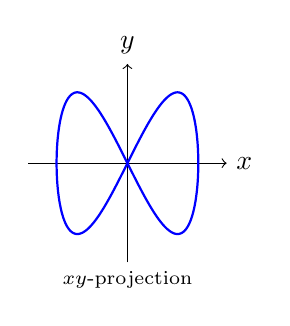
\begin{tikzpicture}[scale=0.9]
\draw[->] (-1.4,0) -- (1.4,0) node[right] {\(x\)};
\draw[->] (0,-1.4) -- (0,1.4) node[above] {\(y\)};
\draw[thick,blue,domain=0:360,samples=240,smooth,variable=\t]
  plot ({sin(\t)},{sin(2*\t)});
\node at (0,-1.65) {\scriptsize \(xy\)-projection};
\end{tikzpicture}

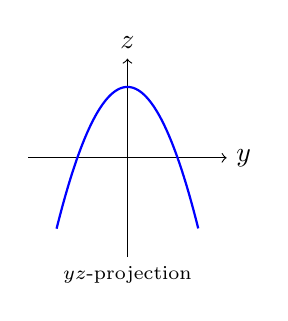
\begin{tikzpicture}[scale=0.9]
\draw[->] (-1.4,0) -- (1.4,0) node[right] {\(y\)};
\draw[->] (0,-1.4) -- (0,1.4) node[above] {\(z\)};
\draw[thick,blue,domain=-1:1,samples=160,smooth,variable=\u]
  plot ({\u},{1-2*(\u)^2});
\node at (0,-1.65) {\scriptsize \(yz\)-projection};
\end{tikzpicture}

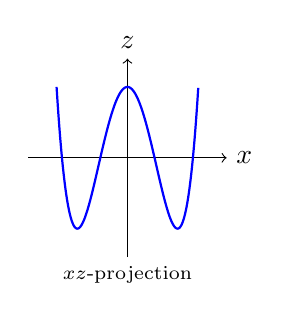
\begin{tikzpicture}[scale=0.9]
\draw[->] (-1.4,0) -- (1.4,0) node[right] {\(x\)};
\draw[->] (0,-1.4) -- (0,1.4) node[above] {\(z\)};
\draw[thick,blue,domain=-1:1,samples=160,smooth,variable=\u]
  plot ({\u},{1-8*(\u)^2+8*(\u)^4});
\node at (0,-1.65) {\scriptsize \(xz\)-projection};
\end{tikzpicture}
\end{center}
\end{solutionbox}

\problem{prob:13-1-57}{57}{The trajectories of two particles are
\[
r_1(t)=\langle t^2,\ 7t-12,\ t^2\rangle,\qquad
r_2(t)=\langle 4t-3,\ t^2,\ 5t-6\rangle,
\]
for \(t\ge 0\). Do the particles collide?}

\begin{solutionbox}
\textbf{Method 1: Set the positions equal at the same time}

\begin{steps}
\item A collision means both particles are at the same point at the same time, so we must solve
\[
r_1(t)=r_2(t)
\]
with the same \(t\).

\item Equating coordinates gives
\[
t^2=4t-3,\qquad
7t-12=t^2,\qquad
t^2=5t-6.
\]
This is appropriate because a collision is coordinatewise equality.

\item Solve each equation:
\[
t^2-4t+3=0 \Rightarrow t=1,3,
\]
\[
t^2-7t+12=0 \Rightarrow t=3,4,
\]
\[
t^2-5t+6=0 \Rightarrow t=2,3.
\]
The common value is
\[
t=3.
\]

\item At \(t=3\),
\[
r_1(3)=\langle 9,9,9\rangle,
\qquad
r_2(3)=\langle 9,9,9\rangle.
\]
So the particles collide at \((9,9,9)\).
\end{steps}
\end{solutionbox}

\begin{solutionbox}
\textbf{Method 2: Use one coordinate to generate candidates and test the rest}

\begin{steps}
\item The \(x\)-coordinates must agree, so begin with
\[
t^2=4t-3.
\]
This is the simplest component equation, and it immediately gives the candidate times
\[
t=1,\ 3.
\]

\item Test these in the other coordinates. For \(t=1\),
\[
7t-12=-5,\qquad t^2=1,
\]
so the \(y\)-coordinates do not match. Hence \(t=1\) is impossible.

\item For \(t=3\),
\[
7t-12=9=t^2,\qquad t^2=9=5t-6.
\]
All three coordinates agree, so \(t=3\) is a collision time.
\end{steps}
\end{solutionbox}

\begin{solutionbox}
\textbf{Hand-in Version}

Set \(r_1(t)=r_2(t)\):
\[
t^2=4t-3,\qquad 7t-12=t^2,\qquad t^2=5t-6.
\]
These give
\[
t=1,3;\qquad t=3,4;\qquad t=2,3.
\]
The common solution is
\[
\boxed{t=3.}
\]
Then
\[
r_1(3)=r_2(3)=\langle 9,9,9\rangle.
\]
Therefore the particles \textbf{do collide}, and the collision point is
\[
\boxed{(9,9,9).}
\]
\end{solutionbox}

\problem{prob:13-1-59}{59}{%
\begin{subparts}
\item Graph the curve
\[
x=\frac{27}{26}\sin 8t-\frac{8}{39}\sin 18t,
\]
\[
y=-\frac{27}{26}\cos 8t+\frac{8}{39}\cos 18t,
\]
\[
z=\frac{144}{65}\sin 5t.
\]
\item Show that the curve lies on the hyperboloid of one sheet \(144x^2+144y^2-25z^2=100\).
\end{subparts}}

\begin{solutionbox}
\textbf{Method 1: Compute the radius \(x^2+y^2\) directly}

\begin{steps}
\item Let
\[
A=\frac{27}{26},\qquad B=\frac{8}{39}.
\]
Then
\[
x=A\sin 8t-B\sin 18t,\qquad
y=-A\cos 8t+B\cos 18t.
\]
To prove the hyperboloid equation, the natural quantity to form is \(x^2+y^2\), because the target equation contains \(x^2+y^2\).

\item Expand:
\[
x^2+y^2=A^2+B^2-2AB\bigl(\sin 8t\sin 18t+\cos 8t\cos 18t\bigr).
\]
Use
\[
\sin \alpha\sin\beta+\cos\alpha\cos\beta=\cos(\alpha-\beta)
\]
to get
\[
x^2+y^2=A^2+B^2-2AB\cos 10t.
\]

\item Rewrite \(\cos 10t=1-2\sin^2 5t\). Then
\[
x^2+y^2={(A-B)}^2+4AB{(\sin 5t)}^2.
\]
Now compute the constants:
\[
A-B=\frac{27}{26}-\frac{8}{39}=\frac56,
\qquad
4AB=4\cdot \frac{27}{26}\cdot\frac{8}{39}=\frac{144}{169}.
\]
So
\[
x^2+y^2=\frac{25}{36}+\frac{144}{169}{(\sin 5t)}^2.
\]

\item Since
\[
z=\frac{144}{65}\sin 5t,
\]
we have
\[
\frac{25}{144}z^2
=\frac{25}{144}\cdot \frac{144^2}{65^2}\sin^2 5t
=\frac{144}{169}\sin^2 5t.
\]
Therefore
\[
x^2+y^2=\frac{25}{36}+\frac{25}{144}z^2.
\]
Multiply by \(144\):
\[
144x^2+144y^2-25z^2=100.
\]
That proves part (b).

\item The same formula also describes the graph in part (a). The radius from the \(z\)-axis is
\[
\rho=\sqrt{x^2+y^2},
\]
so
\[
\rho^2=\frac{25}{36}+\frac{144}{169}\sin^2 5t.
\]
Hence the curve stays on the one-sheet hyperboloid, with
\[
\rho_{\min}=\frac56,\qquad
\rho_{\max}=\frac{97}{78},
\qquad
z_{\max}=\frac{144}{65},
\qquad
z_{\min}=-\frac{144}{65}.
\]
Because \(z\) has frequency \(5\), the curve makes five up-down oscillations before closing.
\end{steps}
\end{solutionbox}

\begin{solutionbox}
\textbf{Method 2: Use a complex-number shortcut for \(x^2+y^2\)}

\begin{steps}
\item Combine \(x\) and \(y\) into one complex expression:
\[
x+iy
=A(\sin 8t-i\cos 8t)+B(-\sin 18t+i\cos 18t).
\]
Using
\[
\sin \theta-i\cos\theta=-ie^{i\theta},
\qquad
-\sin\theta+i\cos\theta=ie^{i\theta},
\]
we obtain
\[
x+iy=i\bigl(Be^{i18t}-Ae^{i8t}\bigr).
\]
This method is appropriate because \(|x+iy|^2=x^2+y^2\), and the complex form packages the trig terms neatly.

\item Now take the modulus squared:
\[
x^2+y^2
=|x+iy|^2
=A^2+B^2-2AB\cos 10t.
\]
From here the same simplification as in Method 1 gives
\[
x^2+y^2=\frac{25}{36}+\frac{144}{169}\sin^2 5t.
\]

\item Since \(z=\frac{144}{65}\sin 5t\), this becomes
\[
x^2+y^2=\frac{25}{36}+\frac{25}{144}z^2.
\]
So the curve lies on
\[
\boxed{144x^2+144y^2-25z^2=100.}
\]

\item Geometrically, this means the curve is a closed oscillating path wrapped around a one-sheet hyperboloid. A good domain is \(0\le t\le 2\pi\), because all frequencies are integers and the curve closes there.
\end{steps}
\end{solutionbox}

\begin{solutionbox}
\textbf{Hand-in Version}

Let
\[
A=\frac{27}{26},\qquad B=\frac{8}{39}.
\]
Then
\[
x^2+y^2=A^2+B^2-2AB\cos 10t
={(A-B)}^2+4AB{(\sin 5t)}^2.
\]
Since
\[
A-B=\frac56,\qquad 4AB=\frac{144}{169},
\]
we get
\[
x^2+y^2=\frac{25}{36}+\frac{144}{169}\sin^2 5t.
\]
Also
\[
z=\frac{144}{65}\sin 5t
\quad\Longrightarrow\quad
\frac{25}{144}z^2=\frac{144}{169}\sin^2 5t.
\]
Hence
\[
x^2+y^2=\frac{25}{36}+\frac{25}{144}z^2,
\]
so
\[
\boxed{144x^2+144y^2-25z^2=100.}
\]

Therefore the curve lies on the one-sheet hyperboloid \(144x^2+144y^2-25z^2=100\). Over \(0\le t\le 2\pi\), it is a closed oscillating curve on that surface, with
\[
\rho_{\min}=\frac56,\qquad
\rho_{\max}=\frac{97}{78},\qquad
z_{\max}=\frac{144}{65},\qquad
z_{\min}=-\frac{144}{65}.
\]

\begin{center}
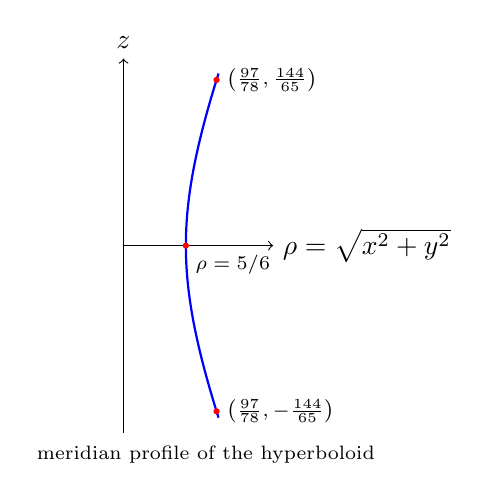
\begin{tikzpicture}[scale=0.95]
\draw[->] (0,0) -- (2.0,0) node[right] {\(\rho=\sqrt{x^2+y^2}\)};
\draw[->] (0,-2.5) -- (0,2.5) node[above] {\(z\)};
\draw[thick,blue,domain=-2.3:2.3,samples=160,smooth,variable=\u]
  plot ({sqrt(25/36 + 25*(\u)^2/144)},{\u});
\fill[red] ({5/6},0) circle (1.2pt);
\node[below right] at ({5/6},0) {\scriptsize \(\rho=5/6\)};
\fill[red] ({97/78},{144/65}) circle (1.2pt);
\fill[red] ({97/78},{-144/65}) circle (1.2pt);
\node[right] at ({97/78},{144/65}) {\scriptsize \(\left(\frac{97}{78},\frac{144}{65}\right)\)};
\node[right] at ({97/78},{-144/65}) {\scriptsize \(\left(\frac{97}{78},-\frac{144}{65}\right)\)};
\node at (1.1,-2.8) {\scriptsize meridian profile of the hyperboloid};
\end{tikzpicture}
\end{center}
\end{solutionbox}

\problem{prob:13-1-60}{60}{Use
\[
x=(2+\cos 1.5t)\cos t,\qquad
y=(2+\cos 1.5t)\sin t,\qquad
z=\sin 1.5t
\]
to sketch the trefoil knot and explain its top view.}

\begin{solutionbox}
\textbf{Method 1: Work in polar coordinates for the top view}

\begin{steps}
\item In the \(xy\)-plane,
\[
x=r\cos\theta,\qquad y=r\sin\theta
\]
with
\[
r=2+\cos 1.5t,\qquad \theta=t.
\]
This is the correct first step because the problem explicitly asks for the view from above, and polar coordinates describe that projection most naturally.

\item Since \(-1\le \cos 1.5t\le 1\),
\[
1\le r\le 3.
\]
So the top-view projection stays between the circles \(r=1\) and \(r=3\).

\item The projection is halfway between \(r=1\) and \(r=3\) when \(r=2\). That means
\[
2+\cos 1.5t=2
\quad\Longrightarrow\quad
\cos 1.5t=0.
\]
Thus
\[
1.5t=\frac{\pi}{2}+k\pi.
\]
At those same parameter values,
\[
z=\sin 1.5t=\pm1.
\]
So the maximum and minimum \(z\)-values occur exactly when the top-view radius is halfway between \(1\) and \(3\).

\item The top-view self-intersections occur precisely at these same points, because if \(r=2\) then the points with parameters \(t\) and \(t+2\pi\) project to the same point in the plane. In one full period \(0\le t\le 4\pi\), the crossings are
\[
(-2,0),\qquad (1,\sqrt3),\qquad (1,-\sqrt3).
\]
At one passage through each crossing, \(z=1\), and at the other, \(z=-1\), so one branch passes over and the other under.
\end{steps}
\end{solutionbox}

\begin{solutionbox}
\textbf{Method 2: Use symmetry and period to understand the whole knot}

\begin{steps}
\item The smallest period of the full space curve is \(4\pi\), because \(\theta=t\) requires a \(2\pi\)-turn in the plane, while \(\cos 1.5t\) and \(\sin 1.5t\) require a common period of \(4\pi\). So \(0\le t\le 4\pi\) gives the entire knot.

\item Now shift the parameter by \(4\pi/3\):
\[
1.5\left(t+\frac{4\pi}{3}\right)=1.5t+2\pi.
\]
Therefore
\[
2+\cos\!\left(1.5\left(t+\frac{4\pi}{3}\right)\right)=2+\cos(1.5t),
\qquad
z\left(t+\frac{4\pi}{3}\right)=z(t).
\]
But the angle in the \(xy\)-plane changes by \(4\pi/3\). So the curve has \(120^\circ\) rotational symmetry about the \(z\)-axis.

\item This explains why the knot has three identical lobes and three crossings in the top view. It is the standard trefoil-knot pattern.

\item Key points support the sketch:
\[
t=0\Rightarrow (3,0,0),\qquad
t=2\pi\Rightarrow (1,0,0),\qquad
t=4\pi\Rightarrow (3,0,0).
\]
Between these, the curve alternately rises above and dips below the \(xy\)-plane, creating the over-under pattern of the knot.
\end{steps}
\end{solutionbox}

\begin{solutionbox}
\textbf{Hand-in Version}

From
\[
x=(2+\cos 1.5t)\cos t,\qquad y=(2+\cos 1.5t)\sin t,
\]
the top-view projection has polar coordinates
\[
\boxed{r=2+\cos 1.5t,\qquad \theta=t.}
\]
Hence
\[
\boxed{1\le r\le 3.}
\]

The radius is halfway between \(1\) and \(3\) when \(r=2\), so \(\cos 1.5t=0\). At these values,
\[
z=\sin 1.5t=\pm1,
\]
so the maximum and minimum values of \(z\) occur exactly when the projection is halfway between the two extreme radii.

The full space curve has period \(4\pi\) and \(120^\circ\) rotational symmetry about the \(z\)-axis, so it is a trefoil knot. The top-view crossings occur at
\[
(-2,0),\qquad (1,\sqrt3),\qquad (1,-\sqrt3),
\]
with one branch above and one branch below at each crossing.

\begin{center}
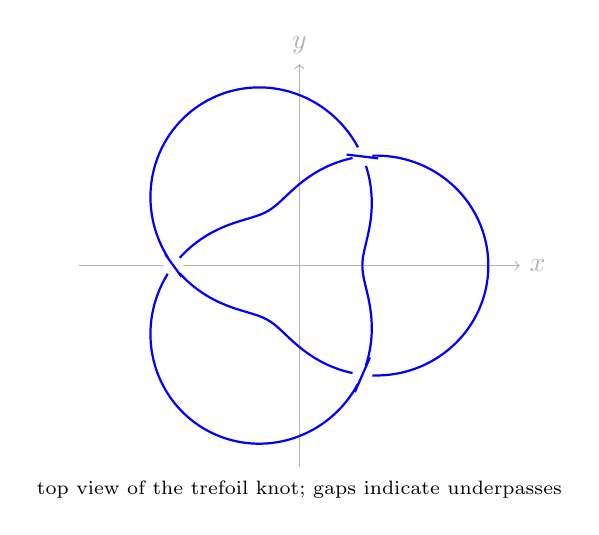
\begin{tikzpicture}[scale=0.8]
\draw[->,gray!60] (-3.5,0) -- (3.5,0) node[right] {\(x\)};
\draw[->,gray!60] (0,-3.2) -- (0,3.2) node[above] {\(y\)};
\draw[thick,blue,domain=0:720,samples=400,smooth,variable=\t]
  plot ({(2+cos(1.5*\t))*cos(\t)},{(2+cos(1.5*\t))*sin(\t)});

\fill[white] (-2,0) circle (0.16);
\fill[white] (1,1.732) circle (0.16);
\fill[white] (1,-1.732) circle (0.16);

\draw[thick,blue] (-2.13,0.18) -- (-1.87,-0.18);
\draw[thick,blue] (0.75,1.762) -- (1.25,1.702);
\draw[thick,blue] (0.88,-2.01) -- (1.12,-1.46);

\node at (0,-3.55) {\scriptsize top view of the trefoil knot; gaps indicate underpasses};
\end{tikzpicture}
\end{center}
\end{solutionbox}

\sectiontitle{sec:13-2}{13-2}

\problem{prob:13-2-24}{24}{If \(r(t)=\langle e^{2t},\ e^{-3t},\ t\rangle\), find \(r'(0)\), \(T(0)\), \(r''(0)\), and \(r'(0)\times r''(0)\).}

\begin{solutionbox}
\textbf{Method 1: Differentiate directly}

\begin{steps}
\item Differentiate once:
\[
r'(t)=\langle 2e^{2t},\ -3e^{-3t},\ 1\rangle.
\]
So
\[
r'(0)=\langle 2,-3,1\rangle.
\]
This is the correct first step because both \(T(0)\) and the cross product require \(r'(0)\).

\item The unit tangent vector is
\[
T(0)=\frac{r'(0)}{|r'(0)|}.
\]
Now
\[
|r'(0)|=\sqrt{2^2+{(-3)}^2+1^2}=\sqrt{14},
\]
so
\[
T(0)=\left\langle \frac{2}{\sqrt{14}},\ -\frac{3}{\sqrt{14}},\ \frac{1}{\sqrt{14}}\right\rangle.
\]

\item Differentiate again:
\[
r''(t)=\langle 4e^{2t},\ 9e^{-3t},\ 0\rangle.
\]
Hence
\[
r''(0)=\langle 4,9,0\rangle.
\]

\item Finally,
\[
r'(0)\times r''(0)
=
\begin{vmatrix}
\mathbf i & \mathbf j & \mathbf k\\
2 & -3 & 1\\
4 & 9 & 0
\end{vmatrix}
=\langle -9,4,30\rangle.
\]
\end{steps}
\end{solutionbox}

\begin{solutionbox}
\textbf{Method 2: Use the coordinate formulas one component at a time}

\begin{steps}
\item The coordinate functions are
\[
x=e^{2t},\qquad y=e^{-3t},\qquad z=t.
\]
Differentiate each separately:
\[
x'=2e^{2t},\quad y'=-3e^{-3t},\quad z'=1,
\]
so at \(t=0\),
\[
r'(0)=\langle 2,-3,1\rangle.
\]

\item Differentiate again:
\[
x''=4e^{2t},\quad y''=9e^{-3t},\quad z''=0,
\]
thus
\[
r''(0)=\langle 4,9,0\rangle.
\]

\item Normalize \(r'(0)\) to get the tangent vector:
\[
T(0)=\frac{\langle 2,-3,1\rangle}{\sqrt{14}}.
\]

\item Then compute the cross product from the two vectors already found:
\[
\langle 2,-3,1\rangle\times \langle 4,9,0\rangle
=\langle -9,4,30\rangle.
\]
This method is appropriate because it keeps the calculation transparent and minimizes the chance of sign errors.
\end{steps}
\end{solutionbox}

\begin{solutionbox}
\textbf{Hand-in Version}

\[
r'(t)=\langle 2e^{2t},-3e^{-3t},1\rangle
\quad\Longrightarrow\quad
\boxed{r'(0)=\langle 2,-3,1\rangle.}
\]

\[
|r'(0)|=\sqrt{14}
\quad\Longrightarrow\quad
\boxed{T(0)=\left\langle \frac{2}{\sqrt{14}},-\frac{3}{\sqrt{14}},\frac{1}{\sqrt{14}}\right\rangle.}
\]

\[
r''(t)=\langle 4e^{2t},9e^{-3t},0\rangle
\quad\Longrightarrow\quad
\boxed{r''(0)=\langle 4,9,0\rangle.}
\]

\[
\boxed{r'(0)\times r''(0)=\langle -9,4,30\rangle.}
\]
\end{solutionbox}

\problem{prob:13-2-28}{28}{Find parametric equations for the tangent line to
\[
x=\sqrt{t^2+3},\qquad y=\ln(t^2+3),\qquad z=t
\]
at the point \((2,\ln 4,1)\).}

\begin{solutionbox}
\textbf{Method 1: Find the parameter first, then use \(r'(t)\)}

\begin{steps}
\item The given point has \(z=1\), and since \(z=t\), the corresponding parameter is
\[
t=1.
\]
This is the correct first step because tangent data from a parametric curve must be evaluated at the correct parameter value.

\item Differentiate:
\[
x'(t)=\frac{t}{\sqrt{t^2+3}},\qquad
y'(t)=\frac{2t}{t^2+3},\qquad
z'(t)=1.
\]
At \(t=1\),
\[
r'(1)=\left\langle \frac12,\frac12,1\right\rangle.
\]

\item Therefore the tangent line through \((2,\ln 4,1)\) is
\[
\ell(s)=\langle 2,\ln 4,1\rangle+s\left\langle \frac12,\frac12,1\right\rangle.
\]
Equivalently, using the direction vector \(\langle 1,1,2\rangle\),
\[
\ell(s)=\langle 2,\ln 4,1\rangle+s\langle 1,1,2\rangle.
\]
\end{steps}
\end{solutionbox}

\begin{solutionbox}
\textbf{Method 2: Use \(z\) itself as the running parameter}

\begin{steps}
\item Because \(z=t\), we may rewrite the curve as
\[
x=\sqrt{z^2+3},\qquad y=\ln(z^2+3),\qquad z=z.
\]
This is appropriate because it turns the third coordinate into the natural parameter.

\item Differentiate with respect to \(z\):
\[
\frac{dx}{dz}=\frac{z}{\sqrt{z^2+3}},\qquad
\frac{dy}{dz}=\frac{2z}{z^2+3},\qquad
\frac{dz}{dz}=1.
\]
At \(z=1\),
\[
\left(\frac{dx}{dz},\frac{dy}{dz},\frac{dz}{dz}\right)=\left(\frac12,\frac12,1\right).
\]

\item So the tangent line through \((2,\ln 4,1)\) is
\[
x=2+\frac{s}{2},\qquad y=\ln 4+\frac{s}{2},\qquad z=1+s.
\]
Scaling the direction vector gives the equivalent form
\[
\boxed{x=2+u,\qquad y=\ln 4+u,\qquad z=1+2u.}
\]
\end{steps}
\end{solutionbox}

\begin{solutionbox}
\textbf{Hand-in Version}

Since \(z=t\), the point \((2,\ln 4,1)\) corresponds to \(t=1\). Then
\[
r'(t)=\left\langle \frac{t}{\sqrt{t^2+3}},\frac{2t}{t^2+3},1\right\rangle
\]
gives
\[
r'(1)=\left\langle \frac12,\frac12,1\right\rangle.
\]
Hence the tangent line is
\[
\boxed{\ell(s)=\langle 2,\ln 4,1\rangle+s\left\langle \frac12,\frac12,1\right\rangle.}
\]
An equivalent parametric form is
\[
\boxed{x=2+u,\qquad y=\ln 4+u,\qquad z=1+2u.}
\]
\end{solutionbox}

\problem{prob:13-2-29}{29}{Find a vector equation for the tangent line to the curve of intersection of the cylinders \(x^2+y^2=25\) and \(y^2+z^2=20\) at \((3,4,2)\).}

\begin{solutionbox}
\textbf{Method 1: Cross the two normal vectors}

\begin{steps}
\item Let
\[
F(x,y,z)=x^2+y^2-25,\qquad G(x,y,z)=y^2+z^2-20.
\]
The intersection curve lies on both surfaces, so its tangent vector must be perpendicular to both gradients. This is why the cross product of the two normals is the natural tool.

\item Compute the normals at \((3,4,2)\):
\[
\nabla F=\langle 2x,2y,0\rangle \Rightarrow \nabla F(3,4,2)=\langle 6,8,0\rangle,
\]
\[
\nabla G=\langle 0,2y,2z\rangle \Rightarrow \nabla G(3,4,2)=\langle 0,8,4\rangle.
\]

\item Their cross product is
\[
\nabla F\times \nabla G
=
\begin{vmatrix}
\mathbf i & \mathbf j & \mathbf k\\
6 & 8 & 0\\
0 & 8 & 4
\end{vmatrix}
=\langle 32,-24,48\rangle.
\]
A simpler direction vector is
\[
\langle 4,-3,6\rangle.
\]

\item Therefore the tangent line is
\[
\boxed{\ell(s)=\langle 3,4,2\rangle+s\langle 4,-3,6\rangle.}
\]
\end{steps}
\end{solutionbox}

\begin{solutionbox}
\textbf{Method 2: Differentiate the two constraint equations}

\begin{steps}
\item Suppose the tangent direction is \(\langle x',y',z'\rangle\). Differentiate
\[
x^2+y^2=25,\qquad y^2+z^2=20
\]
with respect to a curve parameter:
\[
2xx'+2yy'=0,\qquad 2yy'+2zz'=0.
\]
This method is appropriate because it uses the defining equations of the intersection directly.

\item At \((3,4,2)\), these become
\[
3x'+4y'=0,\qquad 4y'+2z'=0.
\]
From the second,
\[
z'=-2y'.
\]
From the first,
\[
x'=-\frac43 y'.
\]

\item Choose \(y'=-3\). Then
\[
x'=4,\qquad z'=6.
\]
So a tangent direction is
\[
\langle 4,-3,6\rangle.
\]
Hence
\[
\boxed{\ell(s)=\langle 3,4,2\rangle+s\langle 4,-3,6\rangle.}
\]
\end{steps}
\end{solutionbox}

\begin{solutionbox}
\textbf{Hand-in Version}

Let
\[
F=x^2+y^2-25,\qquad G=y^2+z^2-20.
\]
Then
\[
\nabla F(3,4,2)=\langle 6,8,0\rangle,\qquad
\nabla G(3,4,2)=\langle 0,8,4\rangle.
\]
A tangent vector is
\[
\nabla F\times \nabla G
=\langle 32,-24,48\rangle
\sim \langle 4,-3,6\rangle.
\]
Therefore the tangent line is
\[
\boxed{\ell(s)=\langle 3,4,2\rangle+s\langle 4,-3,6\rangle.}
\]
\end{solutionbox}

\problem{prob:13-2-35}{35}{The curves
\[
r_1(t)=\langle t,\ t^2,\ t^3\rangle,\qquad
r_2(t)=\langle \sin t,\ \sin 2t,\ t\rangle
\]
intersect at the origin. Find their angle of intersection correct to the nearest degree.}

\begin{solutionbox}
\textbf{Method 1: Use the tangent vectors at the intersection point}

\begin{steps}
\item The angle of intersection of two curves is the angle between their tangent vectors at the common point. This is appropriate because the tangent line is the first-order local model of a curve.

\item Differentiate:
\[
r_1'(t)=\langle 1,2t,3t^2\rangle,
\qquad
r_2'(t)=\langle \cos t,2\cos 2t,1\rangle.
\]
At the origin, both curves correspond to \(t=0\), so
\[
r_1'(0)=\langle 1,0,0\rangle,
\qquad
r_2'(0)=\langle 1,2,1\rangle.
\]

\item Use the dot-product formula:
\[
\cos\theta=\frac{r_1'(0)\cdot r_2'(0)}{|r_1'(0)|\,|r_2'(0)|}
\]
to get
\[
\cos\theta=\frac{1}{1\cdot \sqrt{1^2+2^2+1^2}}=\frac{1}{\sqrt6}.
\]
Therefore
\[
\theta=\cos^{-1}\!\left(\frac{1}{\sqrt6}\right)\approx 65.9^\circ.
\]
So the angle is
\[
\boxed{66^\circ.}
\]
\end{steps}
\end{solutionbox}

\begin{solutionbox}
\textbf{Method 2: Linearize both curves near \(t=0\)}

\begin{steps}
\item Near \(t=0\),
\[
r_1(t)=\langle t,t^2,t^3\rangle \approx \langle t,0,0\rangle,
\]
because the higher powers are much smaller than the linear term. So the first curve is tangent to the \(x\)-axis.

\item For the second curve, use the small-angle approximations
\[
\sin t\approx t,\qquad \sin 2t\approx 2t.
\]
Then
\[
r_2(t)=\langle \sin t,\sin 2t,t\rangle \approx \langle t,2t,t\rangle=t\langle 1,2,1\rangle.
\]
So the second tangent direction is \(\langle 1,2,1\rangle\).

\item The angle between the approximate tangent directions \(\langle 1,0,0\rangle\) and \(\langle 1,2,1\rangle\) is
\[
\cos\theta=\frac{1}{\sqrt6},
\]
which gives
\[
\theta\approx 66^\circ.
\]
This agrees with Method 1.
\end{steps}
\end{solutionbox}

\begin{solutionbox}
\textbf{Hand-in Version}

\[
r_1'(t)=\langle 1,2t,3t^2\rangle,\qquad
r_2'(t)=\langle \cos t,2\cos 2t,1\rangle.
\]
At \(t=0\),
\[
r_1'(0)=\langle 1,0,0\rangle,\qquad
r_2'(0)=\langle 1,2,1\rangle.
\]
So
\[
\cos\theta=\frac{\langle 1,0,0\rangle\cdot \langle 1,2,1\rangle}{1\cdot \sqrt6}
=\frac{1}{\sqrt6}.
\]
Hence
\[
\theta=\cos^{-1}\!\left(\frac{1}{\sqrt6}\right)\approx 65.9^\circ.
\]
Therefore the angle of intersection is
\[
\boxed{66^\circ.}
\]
\end{solutionbox}

\problem{prob:13-2-52}{52}{If \(r(t)=u(t)\times v(t)\), where
\[
u(2)=\langle 1,2,-1\rangle,\qquad
u'(2)=\langle 3,0,4\rangle,\qquad
v(t)=\langle t,t^2,t^3\rangle,
\]
find \(r'(2)\).}

\begin{solutionbox}
\textbf{Method 1: Use the product rule for a cross product}

\begin{steps}
\item Since
\[
r(t)=u(t)\times v(t),
\]
differentiate using the vector product rule:
\[
r'(t)=u'(t)\times v(t)+u(t)\times v'(t).
\]
This is the correct main idea because the cross product behaves like a product under differentiation.

\item First compute
\[
v(2)=\langle 2,4,8\rangle,\qquad
v'(t)=\langle 1,2t,3t^2\rangle,
\qquad
v'(2)=\langle 1,4,12\rangle.
\]

\item Now evaluate the two cross products:
\[
u'(2)\times v(2)
=\langle 3,0,4\rangle\times \langle 2,4,8\rangle
=\langle -16,-16,12\rangle,
\]
\[
u(2)\times v'(2)
=\langle 1,2,-1\rangle\times \langle 1,4,12\rangle
=\langle 28,-13,2\rangle.
\]

\item Add them:
\[
r'(2)=\langle -16,-16,12\rangle+\langle 28,-13,2\rangle
=\boxed{\langle 12,-29,14\rangle.}
\]
\end{steps}
\end{solutionbox}

\begin{solutionbox}
\textbf{Method 2: Differentiate the determinant componentwise}

\begin{steps}
\item Write
\[
r(t)=
\begin{vmatrix}
\mathbf i & \mathbf j & \mathbf k\\
u_1(t) & u_2(t) & u_3(t)\\
t & t^2 & t^3
\end{vmatrix}.
\]
Differentiating componentwise is a second valid method because each component of a cross product is an ordinary scalar expression.

\item Expanding formally,
\[
r(t)=\langle u_2t^3-u_3t^2,\ -(u_1t^3-u_3t),\ u_1t^2-u_2t\rangle.
\]
Differentiate:
\[
r'(t)=\langle u_2't^3+3u_2t^2-u_3't^2-2u_3t,\ -(u_1't^3+3u_1t^2-u_3't-u_3),\ u_1't^2+2u_1t-u_2't-u_2\rangle.
\]

\item Substitute \(t=2\), \(u(2)=\langle 1,2,-1\rangle\), and \(u'(2)=\langle 3,0,4\rangle\):
\[
r'(2)=\langle 0\cdot 8+3\cdot 2\cdot 4-4\cdot 4-2(-1)\cdot 2,\ -(3\cdot 8+3\cdot 1\cdot 4-4\cdot 2-(-1)),\ 3\cdot 4+2\cdot 1\cdot 2-0\cdot 2-2\rangle.
\]
This simplifies to
\[
r'(2)=\langle 12,-29,14\rangle.
\]
\end{steps}
\end{solutionbox}

\begin{solutionbox}
\textbf{Hand-in Version}

Since \(r(t)=u(t)\times v(t)\),
\[
r'(t)=u'(t)\times v(t)+u(t)\times v'(t).
\]
Now
\[
v(2)=\langle 2,4,8\rangle,\qquad v'(2)=\langle 1,4,12\rangle.
\]
So
\[
u'(2)\times v(2)
=\langle 3,0,4\rangle\times \langle 2,4,8\rangle
=\langle -16,-16,12\rangle,
\]
\[
u(2)\times v'(2)
=\langle 1,2,-1\rangle\times \langle 1,4,12\rangle
=\langle 28,-13,2\rangle.
\]
Hence
\[
r'(2)=\langle -16,-16,12\rangle+\langle 28,-13,2\rangle
=\boxed{\langle 12,-29,14\rangle.}
\]
\end{solutionbox}

\end{document}
